
\section{Introduction}

Early fundus screening is an effective approach for ocular disease diagnosis, as it can reveal diverse pathological signs in the retina, optic disc, blood vessels, and macular region. Analyzing fundus images helps identify potential lesions and supports early intervention, thereby reducing the risk of irreversible visual impairment or even vision loss. As fundus screening continues to expand, manual fundus screening is limited by its time cost, dependence on expert experience, and shortage of primary medical resources. Fundus-image-based ocular disease diagnosis therefore has important practical value\hyperref[_Ref213949315]{{[}1{]}}. Existing methods for fundus screening can be broadly grouped into three technical directions: ML, VLM, and CNN. ML methods usually rely on hand-crafted features such as image enhancement, lesion segmentation, texture, or morphology, followed by classifiers such as support vector machines or random forests for recognition\hyperref[_RefRahman2022MLFundus]{{[}2{]}}. These methods offer a degree of interpretability, but their feature design depends heavily on prior experience and has limited capacity to represent complex fundus lesions and multi-disease co-occurrence. In recent years, VLM has opened new directions for fundus image understanding, image-text joint analysis, and medical report generation\hyperref[_RefLim2024VLVOphthalmology]{{[}3{]}}\hyperref[_RefUrooj2025LLMMedicalImage]{{[}4{]}}. However, their training and fine-tuning generally require large-scale high-quality annotations, paired image-text data, and substantial computational resources, which remain costly when medical data are scarce, privacy is restricted, and clinical deployment resources are limited. In contrast, CNN-based deep visual models can directly learn local textures, lesion regions, and spatial structural features from fundus images, and have been widely applied to disease recognition\hyperref[_Ref213871637]{{[}5{]}}, lesion segmentation\hyperref[_Ref213948625]{{[}6{]}}, medical image reconstruction\hyperref[_Ref213948898]{{[}7{]}}, and diagnosis and prediction of ocular diseases\hyperref[_Ref213949262]{{[}8{]}}. Therefore, we adopt CNN as the main modeling backbone for multi-label ocular disease recognition. Nevertheless, in real-world clinical deployment, CNN-based ocular disease recognition methods still face challenges including multi-disease co-occurrence, degraded generalization performance across institutions, and privacy preservation. Specifically:

1. In clinical ocular disease diagnosis, a single eye may present multiple diseases simultaneously. Using a standard single-label classifier, or modeling different diseases as fully independent, can therefore lead to false positives and false negatives\hyperref[_Ref213949362]{{[}9{]}}. Multi-label recognition has also been widely studied for natural images. For example, ML-GCN\hyperref[_Ref213949382]{{[}10{]}} constructs graph relevance from label occurrence frequencies, making relevant labels more likely to be recognized once a given label is identified and thereby reducing false negatives. However, in multi-label ocular disease recognition, disease relevance is more complex, and methods that infer disease relevance solely from label frequencies may be unreliable. For multi-disease co-occurrence in fundus images, a more reliable method for label-feature relevance construction is therefore needed.

2. Medical images differ from natural images because their annotations usually require professional physicians, making both data acquisition and annotation costly. In addition, data sharing restrictions and inconsistent label spaces across medical institutions often limit access to multi-source-domain data and collaborative training. Even when a model performs well on the training set of one medical institution, applying it to another institution can introduce domain shift in the target domain because of differences in imaging devices, illumination conditions, and manual processing procedures\hyperref[_Ref213949348]{{[}11{]}}, resulting in performance degradation. As shown in \hyperref[fig:intro-domain-gap]{Fig.~\ref*{fig:intro-domain-gap}.a1} and \hyperref[fig:intro-domain-gap]{Fig.~\ref*{fig:intro-domain-gap}.a3}, the distributions of the source domain and target domain differ. The decision boundary learned by a base model trained only on the source domain (\hyperref[fig:intro-domain-gap]{Fig.~\ref*{fig:intro-domain-gap}.b1}) may not fit the target-domain distribution (\hyperref[fig:intro-domain-gap]{Fig.~\ref*{fig:intro-domain-gap}.b2}). Common domain adaptation (DA) methods align domain distributions by jointly using source-domain and target-domain data during model training\hyperref[_Ref213949354]{{[}12{]}}, but this requires access to target-domain data during training. Although multi-source domain generalization methods avoid access to the target domain, they usually rely on joint training across multiple source domains. In practical settings where collaborative training with medical data is restricted, these assumptions are often hard to meet. Therefore, exploring single domain generalization methods that extract domain-invariant features using only a single source domain better matches the needs of cross-institutional deployment.

\begin{figure}[!htb]
\centering
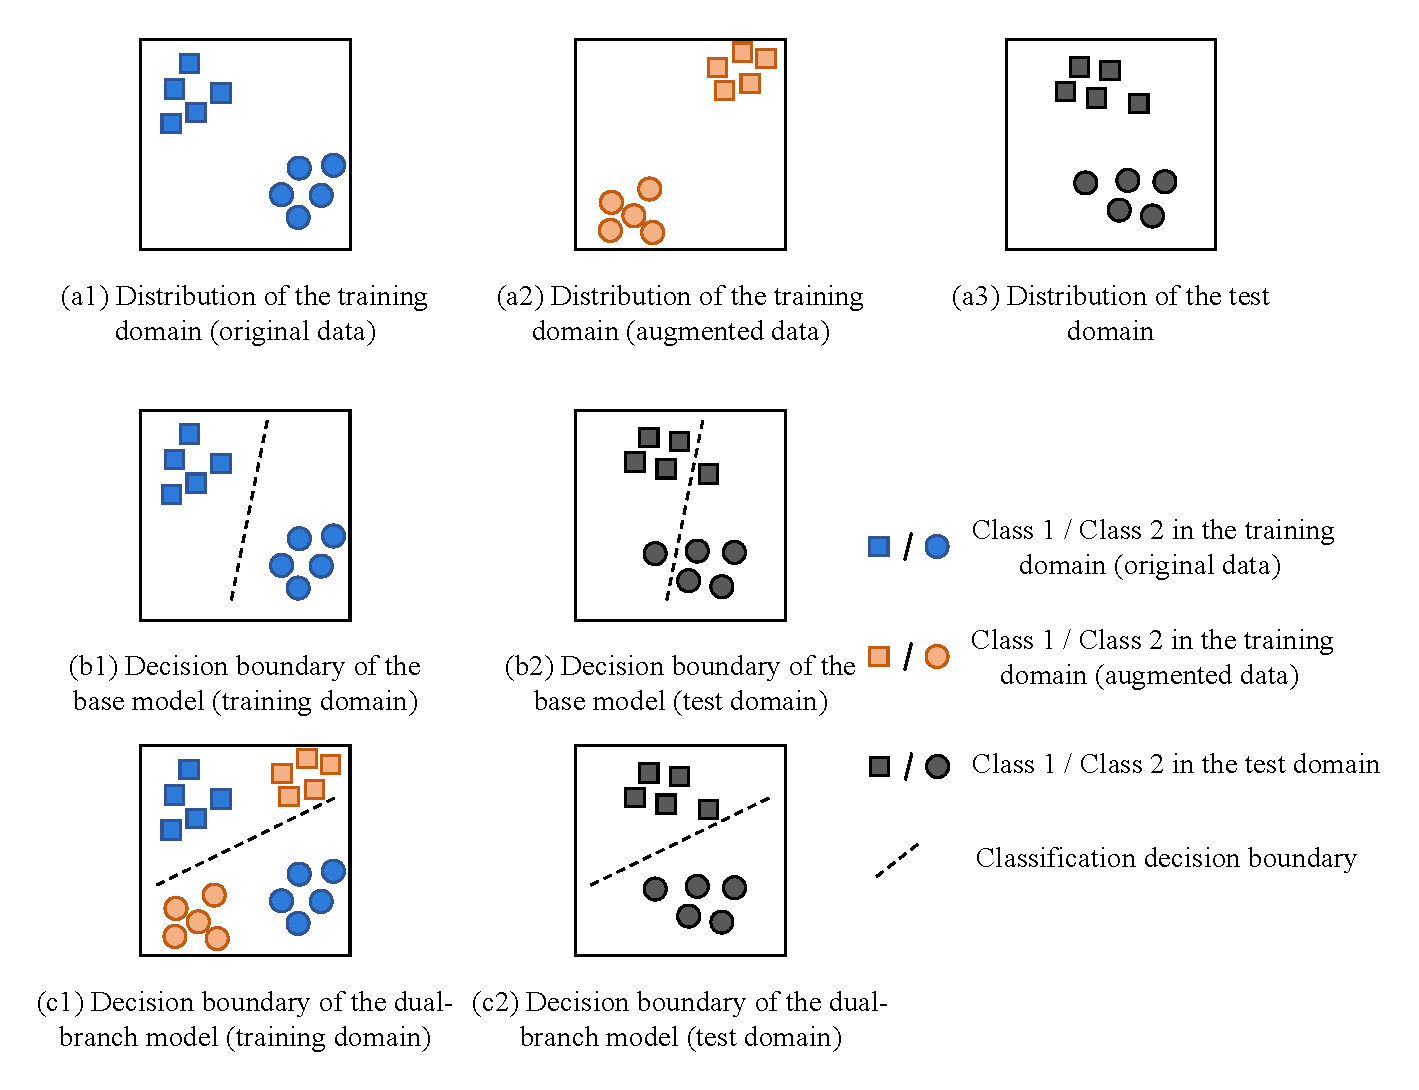
\includegraphics[width=0.72\textwidth]{./images/media/image1_padded.pdf}
\caption{Schematic illustration of the decision boundaries of a conventional model and a dual-branch model under domain shift. (a) shows the distribution relationship among original source-domain images (training set), augmented source-domain images, and the target domain (test set), where augmented source-domain images are used to simulate possible distribution shifts in the target domain. (b) When the model is trained only with original source-domain images, the learned decision boundary may not fit the target domain and can therefore cause classification errors on target-domain samples. (c) By constructing a dual-branch structure with original and augmented source-domain images and incorporating contrastive learning with CAM guidance, the model extracts domain-invariant features and learns a decision boundary that is more applicable to unseen domains.}
\label{fig:intro-domain-gap}
\end{figure}

3. Medical data are more sensitive than natural images and therefore involve higher privacy leakage risk. Common attack methods can recover patient data from model training gradients\hyperref[_Ref213949393]{{[}13{]}}. To address this issue, privacy-preserving methods such as federated learning, homomorphic encryption, secure multi-party computation, and differential privacy have been investigated. However, privacy preservation usually comes with a privacy-performance trade-off. In DA scenarios in particular, source-domain and target-domain data must participate in training simultaneously, which can complicate the integration of privacy mechanisms and cause more severe performance degradation across domains. It is therefore necessary to further explore how to balance privacy preservation and model performance within the single domain generalization training process.

To address the above three key challenges, we build a privacy-preserving interpretable single domain generalization framework for multi-label ocular disease recognition. For the common issue of multi-disease co-occurrence in ocular disease recognition, we introduce a Transformer-based Adaptive Label-Feature Relevance Construction (ARC) module. It models label relevance using Transformer self-attention and fuses label semantics with corresponding image features using Transformer cross-attention, thereby constructing disease co-occurrence dependencies at both the label and feature levels to reduce false positives and false negatives in multi-label recognition. To handle restricted multi-institutional data access together with cross-institutional domain shift, we propose a Dual-Branch Guided Domain-Invariant Feature Extraction (DFE) module. This module is trained using only a single source domain and constructs a dual-branch structure from original source-domain images and style-disturbed augmented source-domain images, as shown in \hyperref[fig:intro-domain-gap]{Fig.~\ref*{fig:intro-domain-gap}.a1} and \hyperref[fig:intro-domain-gap]{Fig.~\ref*{fig:intro-domain-gap}.a2}, to learn their shared representations at the feature level. Meanwhile, Class Activation Mapping (CAM) is introduced as prior guidance to encourage the model to focus on disease-related regions and suppress the learning of domain-specific noise. This enables the model to form a decision boundary that is more suitable for unseen-domain distributions (\hyperref[fig:intro-domain-gap]{Fig.~\ref*{fig:intro-domain-gap}.c1}) and to maintain stable recognition performance on unseen domains (\hyperref[fig:intro-domain-gap]{Fig.~\ref*{fig:intro-domain-gap}.c2}). In addition, CAM visualizes model-attended regions and enhances model interpretability. To address privacy leakage risk in cross-domain medical scenarios, we integrate an Adaptive Gaussian Differential Privacy (AdaGDP) mechanism into the single domain generalization training process and provide privacy preservation by injecting noise during gradient updates. Under a moderate privacy budget, this mechanism preserves privacy without substantially sacrificing model performance, thereby jointly supporting cross-domain generalization and privacy preservation.

Finally, generalization experiments on several representative fundus image datasets show that the framework improves cross-domain multi-label recognition performance while maintaining good interpretability, and it remains stable under privacy-preserving scenarios.

The main contributions of this study are summarized as follows:

\begin{sloppypar}

1. We propose an Adaptive Label-Feature Relevance Construction (ARC) module. Based on Transformer self-attention and cross-attention mechanisms, ARC models disease co-occurrence dependencies at both the label and feature levels, effectively reducing false positives and false negatives in multi-label ocular disease recognition.

2. We design a Dual-Branch Guided Domain-Invariant Feature Extraction (DFE) module. For scenarios where joint training with multi-institutional data is restricted and cross-institutional deployment involves domain shift, this module learns domain-invariant features from a single source domain through joint guidance from style disturbance and CAM. It improves generalization performance on unseen domains and enhances the interpretability of model predictions.

3. We integrate an Adaptive Gaussian Differential Privacy (AdaGDP) mechanism into the single domain generalization training process. Without introducing target-domain data, the proposed mechanism achieves an effective balance between privacy preservation and cross-domain generalization performance, and shows that model performance can remain close to the non-private baseline under moderate privacy preservation.
\end{sloppypar}

The remainder of this paper is organized as follows. Section 2 reviews recent related work. Section 3 presents the proposed method in detail, and Section 4 reports the complete experimental settings and results. Section 5 concludes the paper and discusses future work.
